\chapter{Monitoring the position of the VELO}
\label{chp:pos_VELO}
%\epigraph{With him it is standing on its head. It must be turned right side up again, if you would discover the rational kernel within the mystical shell.}{\textit{Karl Marx} on Hegel}

By leveraging PCA on the 208 cluster counters, we have developed a technique to estimate the position of the beamline with respect to the VELO in Chpater \ref{chap:beamline}. If we make the conceptual exercise of inverting the problem, we can think of this estimator as the position of the VELO relative to a fixed position of the beamline. If we further develop this exercise, we can find a way to estimate the position of two halves of the VELO, referred to as VELO A and VELO C, which move independently. 

Our strategy involves creating six estimators $\hat{x}_A$, $\hat{y}_A$, $\hat{z}_A$, $\hat{x}_C$, $\hat{y}_C$, $\hat{z}_C$, by using a similar technique as the one described in the previous chapter. We achieve this by considering only the 104 counters associated with each half of the VELO, computing the weight vectors by training a PCA model on these counters. This approach provides a robust and flexible way to track the position of the two VELO separately in real time, offering insight into potential detector misalignments and enabling corrections where necessary. Additionally, the urgency of this approach stems from observed drift in one of the VELO halves, making it imperative to have a reliable method to monitor and correct for misalignments.

Throughout this chapter, we will describe the implementation of these new estimators, detailing the selection of relevant cluster counters, the calculation of the corresponding weight vectors on Monte Carlo leveraging the PCA technique and a calibration performed on real data.

Finally, we present the drift of the VELO observed in one of the initial fills of 2024, as a test of the estimators performances.




\section{Estimation of the weights on MC}
As shown in Figure \ref{fig:VELO-counters}, the counters are positioned symmetrically throughout the VELO. Particularly, on each VELO station there are 4 counters on each side of the VELO. By selecting only the 104 counters relative to one side of the VELO, we can train a PCA on these counters to perform an estimation of this VELO side position in the $x$, $y$ and $z$ component, assuming a fixed beamline. This can be sone using the same Monte Carlo simulations and the same approach used in the previous chapter. Although the available MC simulations are made shifting the luminous region, in the assumption of a fixed beamline position, these shifts can be interpreted as a movement of the VELO. By creating 6 different datasets, one for each combination of position $x,y,z$ and VELO side A and C, we can create the 6 estimators $\hat{x}_A$, $\hat{y}_A$, $\hat{x}_C$, $\hat{y}_C$. 

Since the procedure is the same as the one explained in the previous chapter we do not report it once again, but we report the comparison between the scores $\mathbf{t}^{j,s}_{(1)}$ and the relative ``true" position $j=x,y,z$ for each side $s=$A,C of the VELO. We report in the Figures \ref{fig:x_veloA_MC}, \ref{fig:y_veloA_MC}, \ref{fig:x_veloC_MC}, \ref{fig:y_veloC_MC} the scatter plot relative to the estimators $\hat{x}_A$, $\hat{y}_A$, $\hat{x}_C$, $\hat{y}_C$, respectively.
\begin{figure}
    \centering
    \begin{subfigure}{0.48\textwidth}
    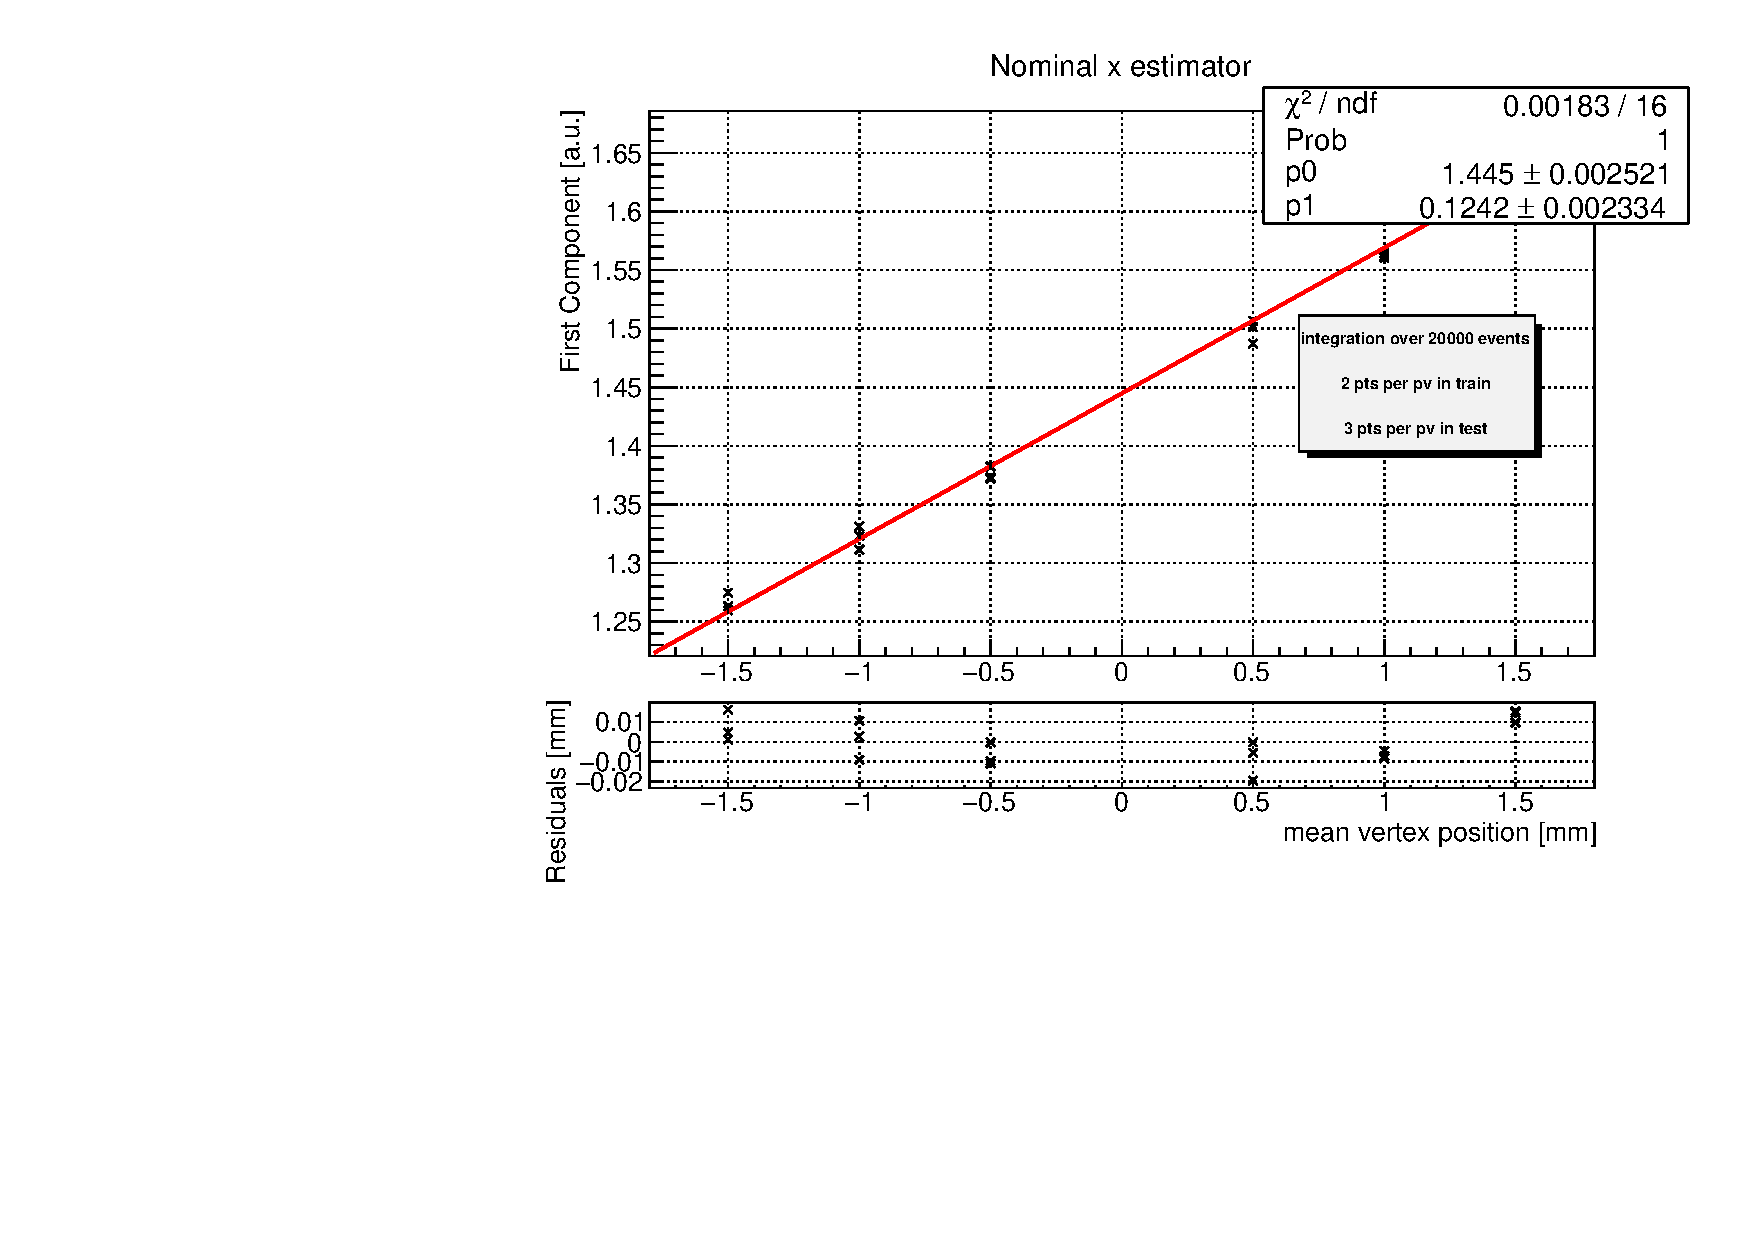
\includegraphics[width=\linewidth]{figures/x_estimate_veloA_MC.pdf}
    \caption{Linear Fit}\label{fig:x_veloA_fit_MC}
    \end{subfigure}
    \begin{subfigure}{0.48\textwidth}
    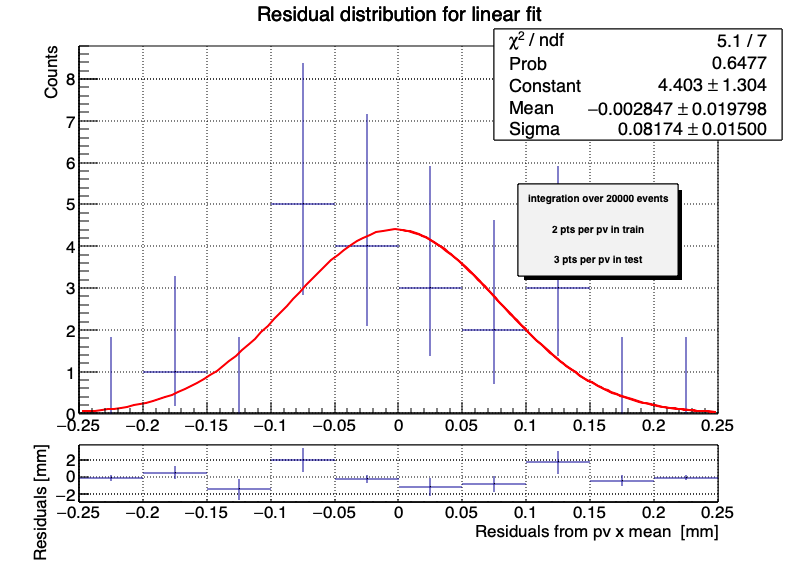
\includegraphics[width=\linewidth]{figures/x_res_veloA_MC.png}
    \caption{Residuals from the fit of the graph on the left. }\label{fig:x_veloA_res_MC}
    \end{subfigure}
    \caption{Linearity of the first component calculated with the PCA with respect to virtual VELO A position shifts in x component, alongside the residuals distribution fitted with a Gaussian distribution.}
    \label{fig:x_veloA_MC}
\end{figure}


\begin{figure}
    \centering
    \begin{subfigure}{0.48\textwidth}
    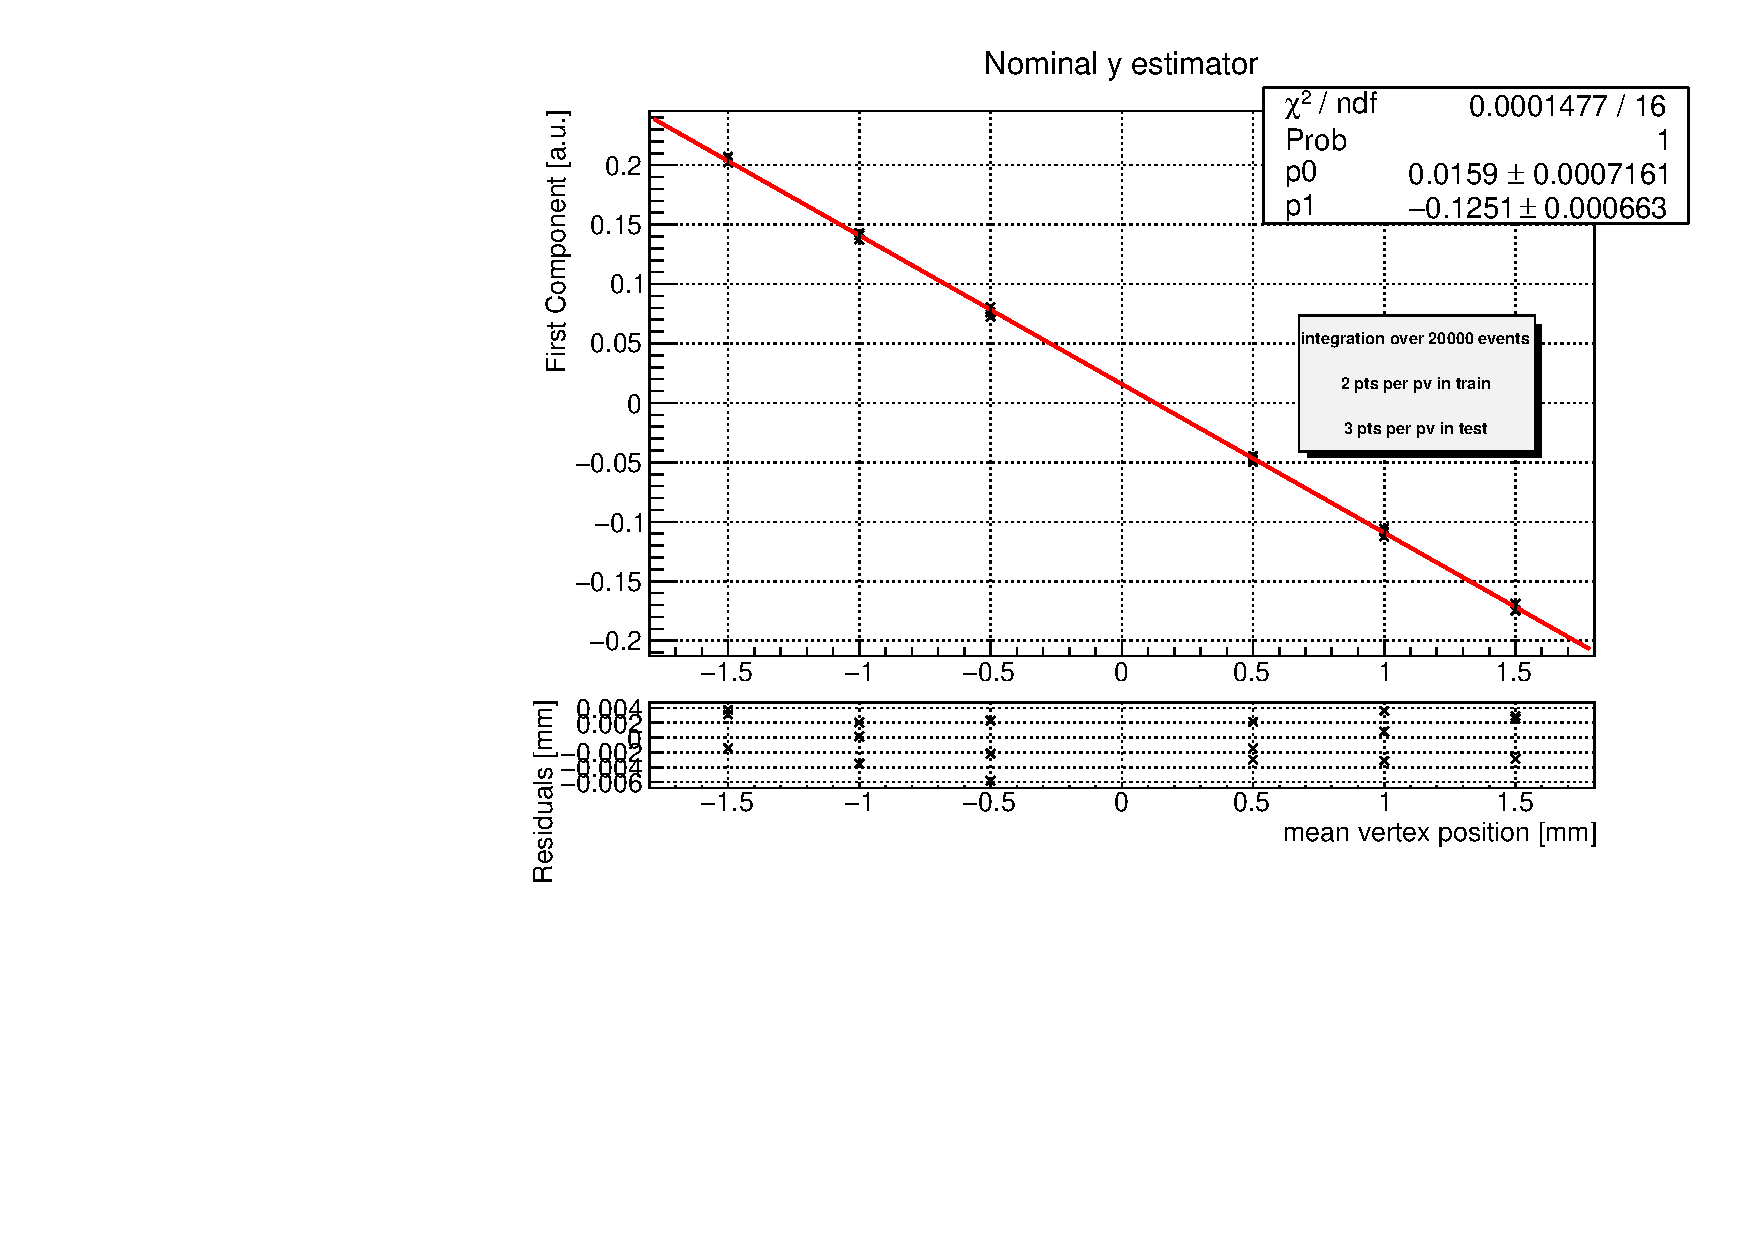
\includegraphics[width=\linewidth]{figures/y_estimate_veloA_MC.pdf}
    \caption{Linear Fit}\label{fig:y_veloA_fit_MC}
    \end{subfigure}
    \begin{subfigure}{0.48\textwidth}
    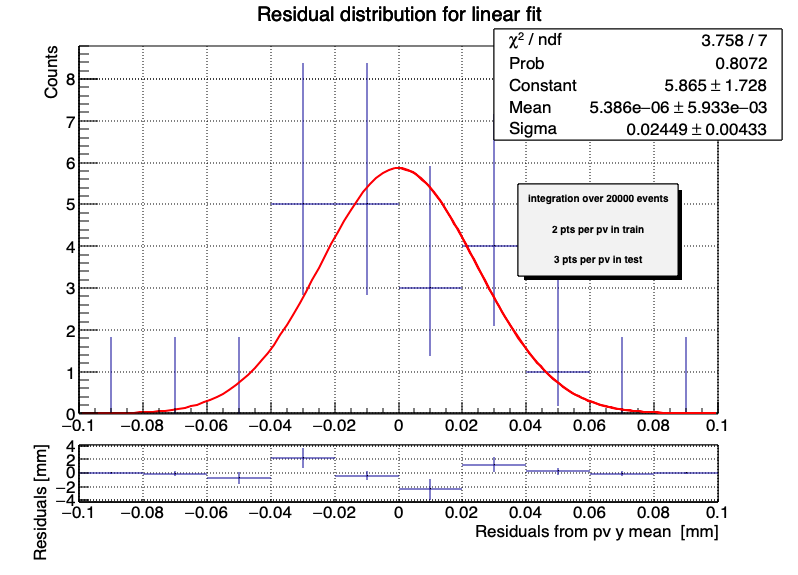
\includegraphics[width=\linewidth]{figures/y_res_veloA_MC.png}
    \caption{Residuals from the fit of the graph on the left. }\label{fig:y_veloA_res_MC}
    \end{subfigure}
    \caption{Linearity of the first component calculated with the PCA with respect to virtual VELO A position shifts in y component, alongside the residuals distribution fitted with a Gaussian distribution.}
    \label{fig:y_veloA_MC}
\end{figure}



\begin{figure}
    \centering
    \begin{subfigure}{0.48\textwidth}
    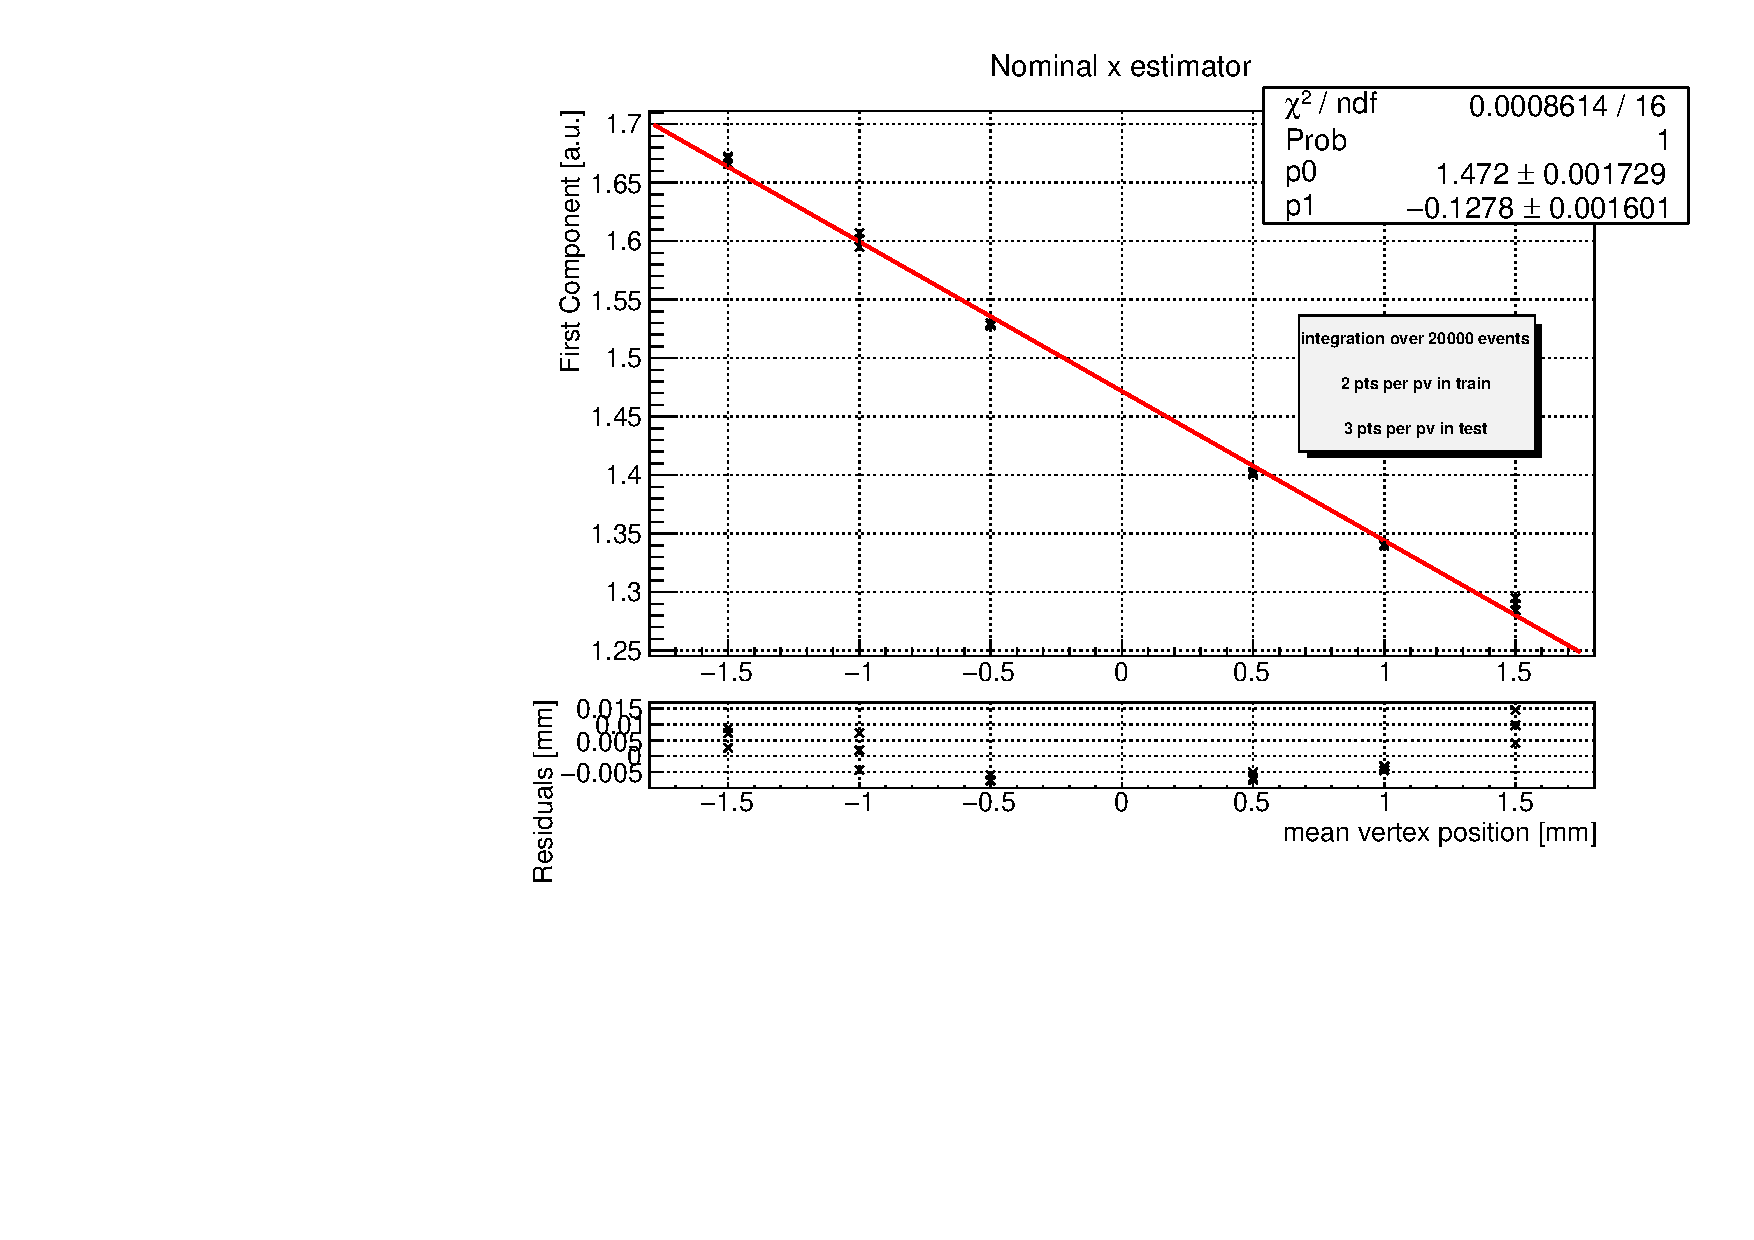
\includegraphics[width=\linewidth]{figures/x_fit_veloC_MC.pdf}
    \caption{Linear Fit}\label{fig:x_veloC_fit_MC}
    \end{subfigure}
    \begin{subfigure}{0.48\textwidth}
    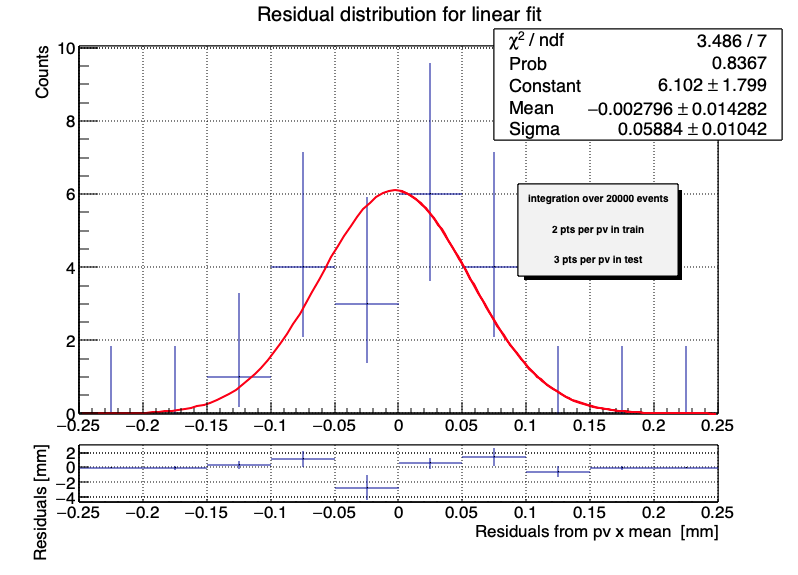
\includegraphics[width=\linewidth]{figures/x_res_veloC_MC.png}
    \caption{Residuals from the fit of the graph on the left. }\label{fig:x_veloC_res_MC}
    \end{subfigure}
    \caption{Linearity of the first component calculated with the PCA with respect to  virtual VELO C position shifts in x component, alongside the residuals distribution fitted with a Gaussian distribution.}
    \label{fig:x_veloC_MC}
\end{figure}
\begin{figure}
    \centering
    \begin{subfigure}{0.48\textwidth}
    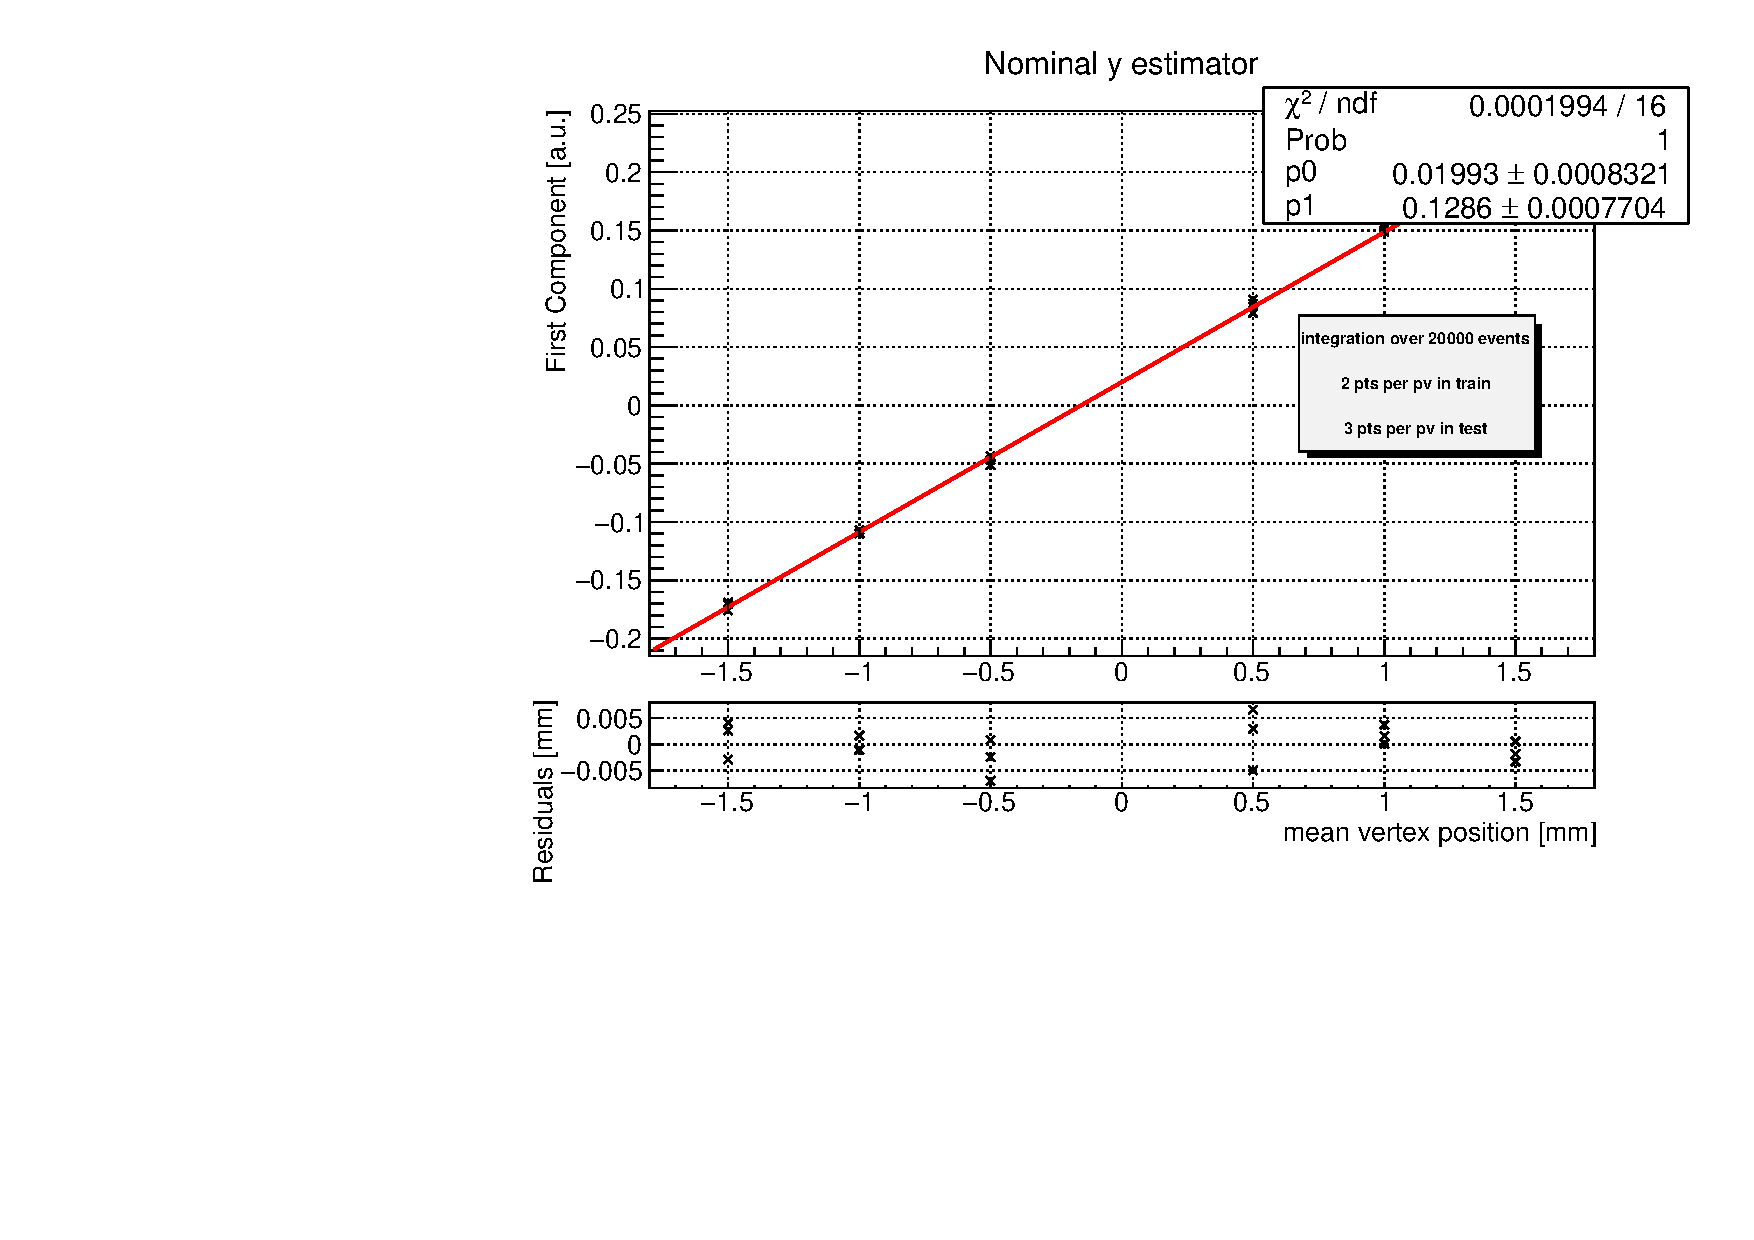
\includegraphics[width=\linewidth]{figures/y_fit_veloC_MC.pdf}
    \caption{Linear Fit}\label{fig:y_veloC_fit_MC}
    \end{subfigure}
    \begin{subfigure}{0.48\textwidth}
    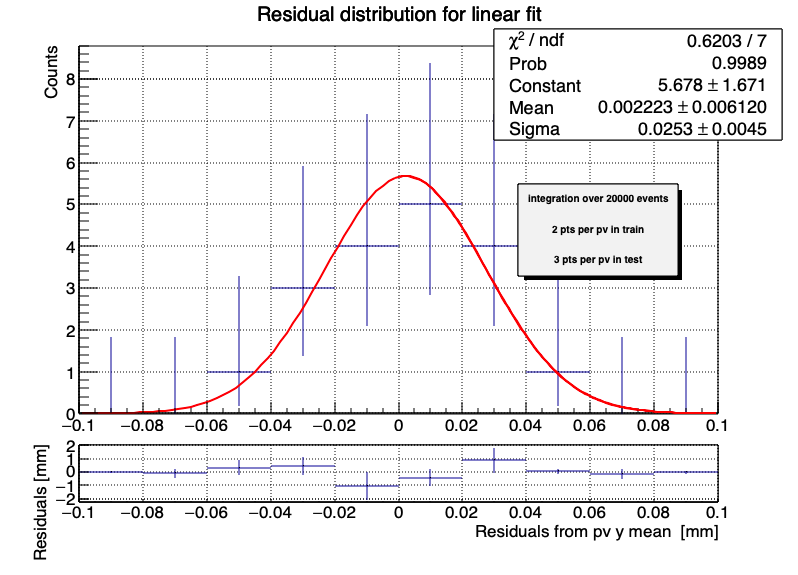
\includegraphics[width=\linewidth]{figures/y_res_veloC_MC.png}
    \caption{Residuals from the fit of the graph on the left. }\label{fig:y_veloC_res_MC}
    \end{subfigure}
    \caption{Linearity of the first component calculated with the PCA with respect to  virtual VELO C position shifts in y component, alongside the residuals distribution fitted with a Gaussian distribution.}
    \label{fig:y_veloC_MC}
\end{figure}

As one can see, there is still a linear relationship between the scores and the virtual VELO positions, showing that the first score is still sufficient to estimate these quantities. Furthermore, the Sigma estimated from the Gaussian fitted in the residuals histogram shows that we are still in the tens of micron range of resolutions, promising good results on the data.


\section{Calibration on real data}
For the calibration we rely directly on real data, using once again the mini VdM performed on April 6th, 2024. 
Once again, we perform the exercise of of thinking the beamline as fixed in space and the VELO moving with respect to this reference. By doing so, we can use the same ramps that were used to calibrate the beamline estimators in the previous chapter. For the comparison, we rely on the reconstructed position of the VELO halves provided by the monitoring tasks of the VELO system. 

\begin{figure}
    \centering
    \begin{subfigure}{0.48\textwidth}
    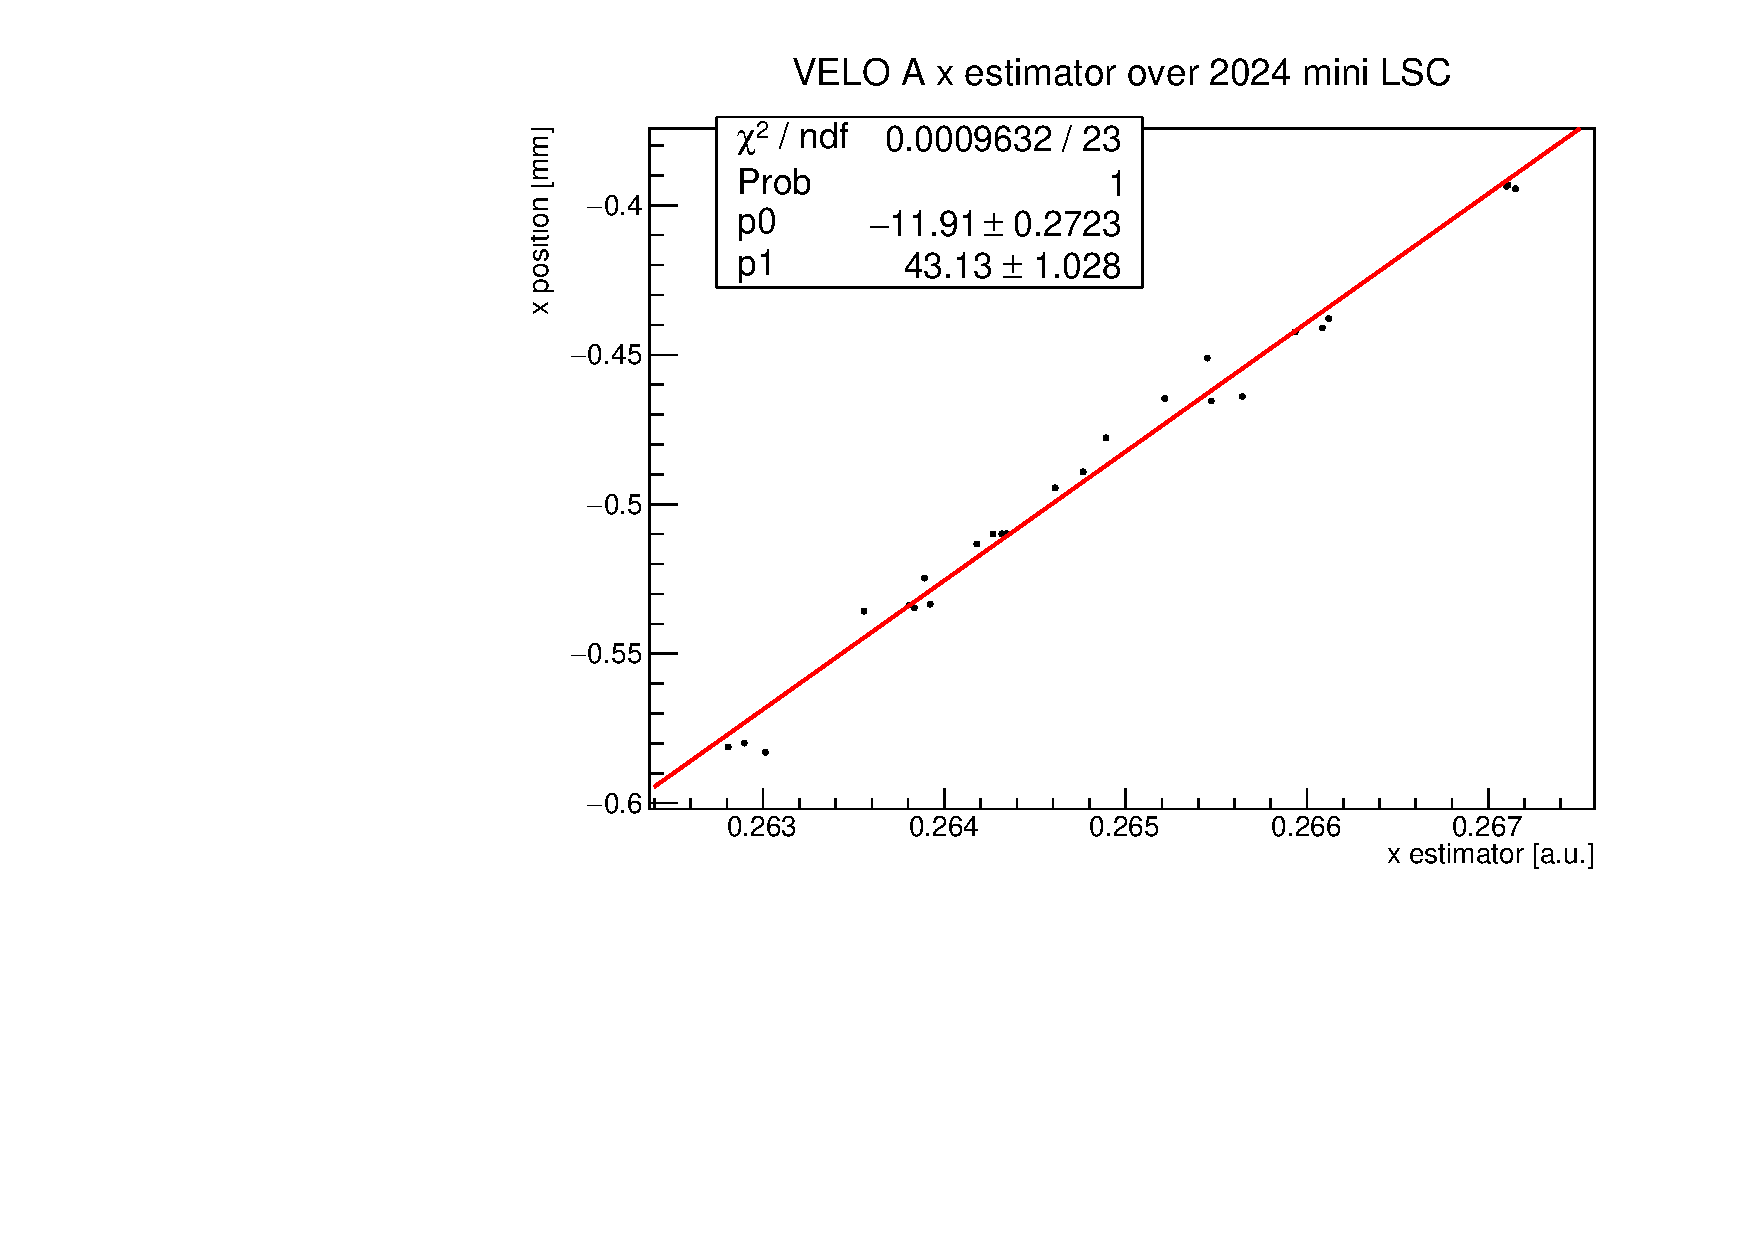
\includegraphics[width=\linewidth]{figures/x_fit_VELO_A_data.pdf}
    \caption{Linear Fit}\label{fig:x_veloA_fit_data}
    \end{subfigure}
    \begin{subfigure}{0.48\textwidth}
    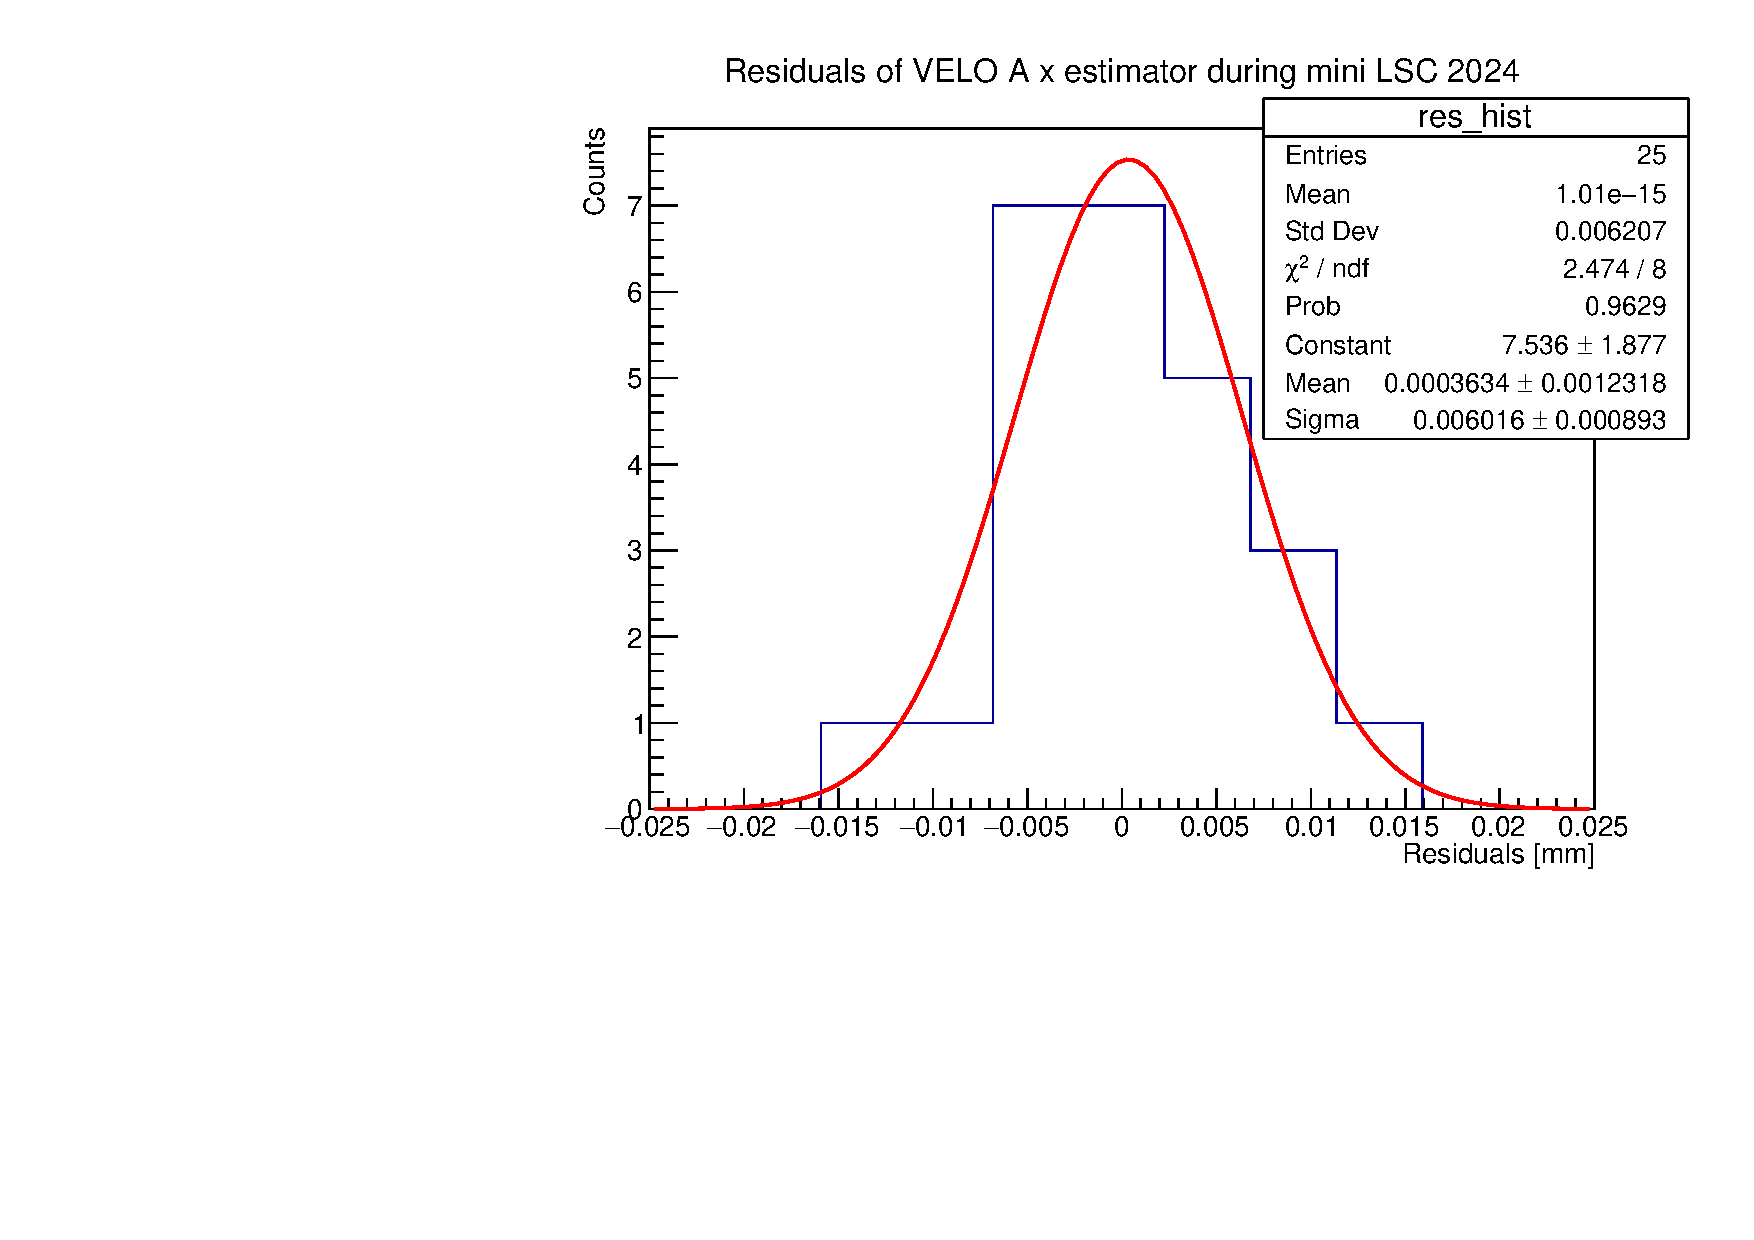
\includegraphics[width=\linewidth]{figures/x_res_VELO_A_data.pdf}
    \caption{Residuals from the fit of the graph on the left. }\label{fig:x_veloA_res_data}
    \end{subfigure}
    \caption{Linearity of the first component calculated with the PCA with respect to virtual VELO A position shifts in x component, alongside the residuals distribution fitted with a Gaussian distribution.}
    \label{fig:x_veloA_data}
\end{figure}


\begin{figure}
    \centering
    \begin{subfigure}{0.48\textwidth}
    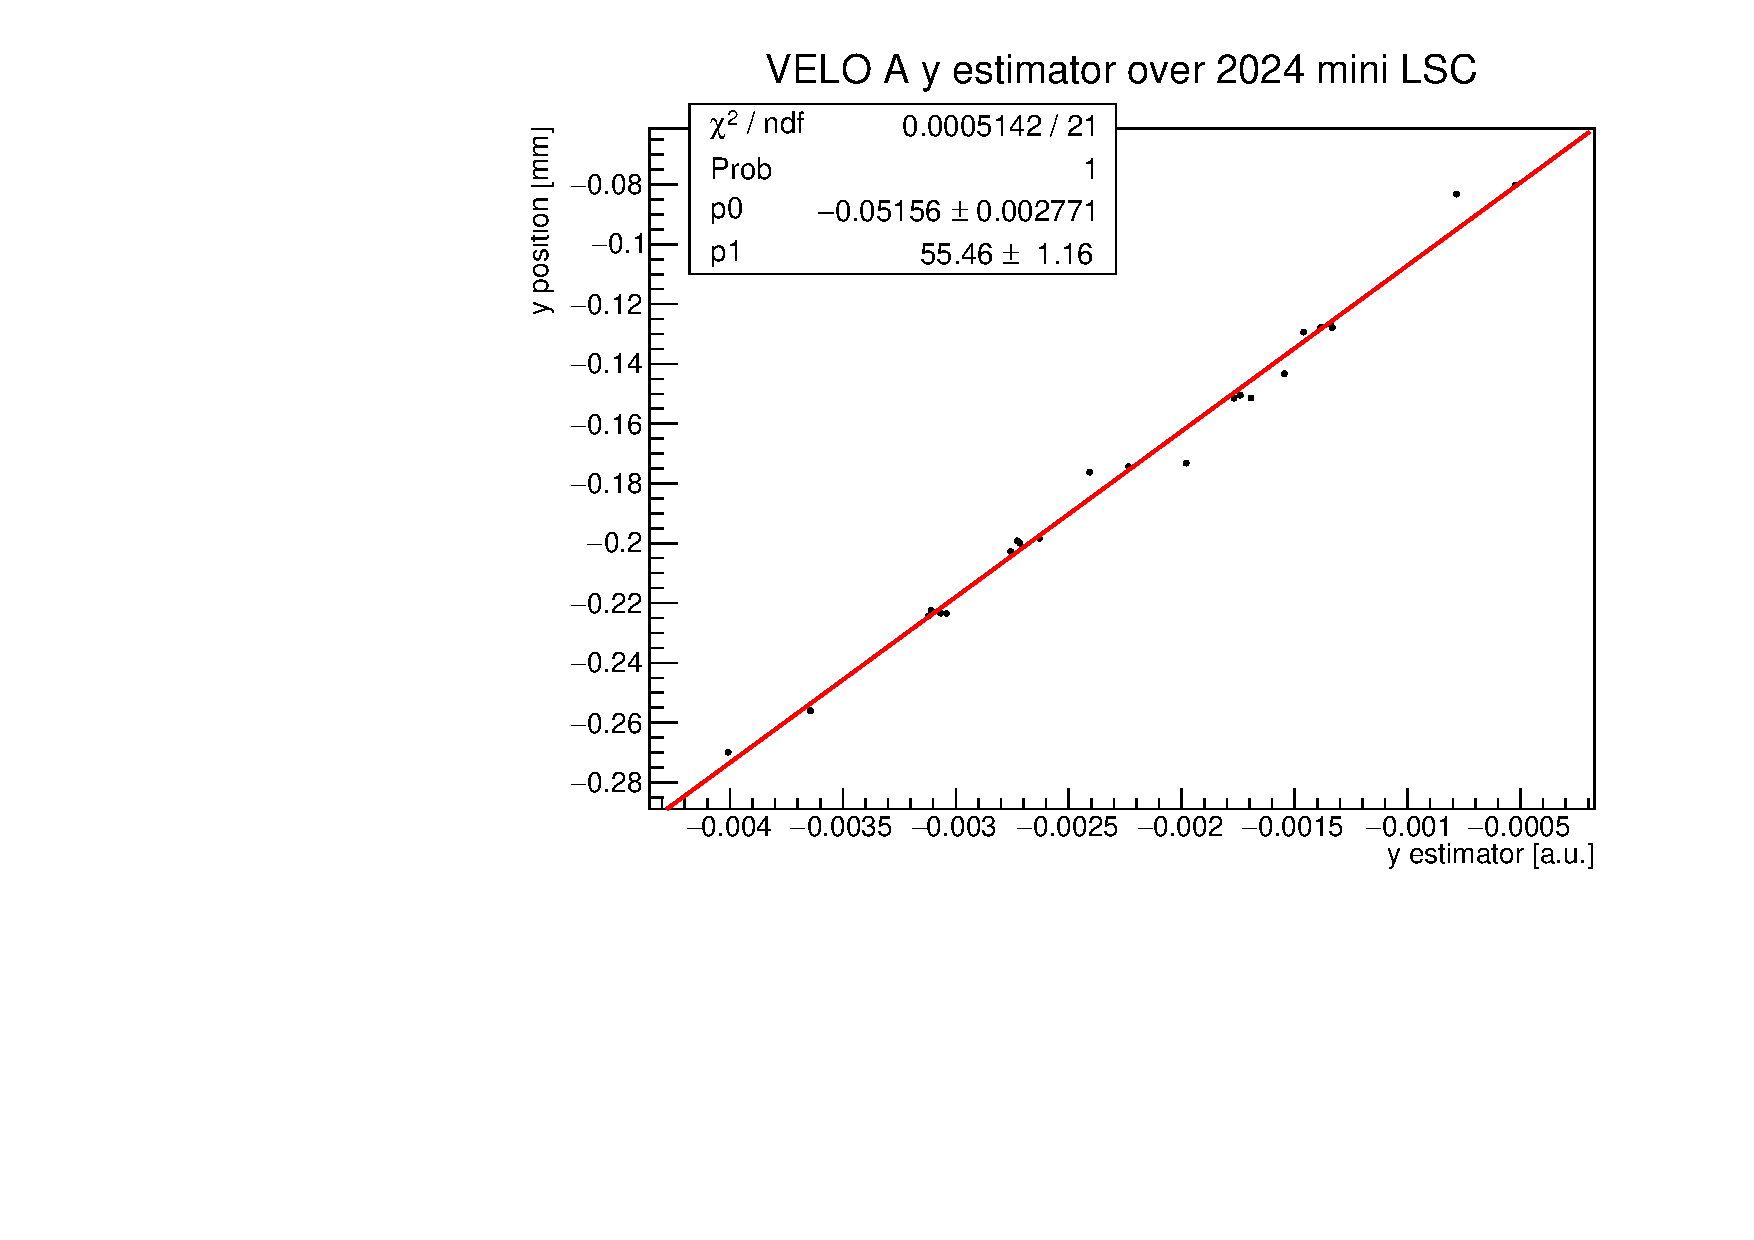
\includegraphics[width=\linewidth]{figures/y_fit_VELO_A_data.pdf}
    \caption{Linear Fit}\label{fig:y_veloA_fit_data}
    \end{subfigure}
    \begin{subfigure}{0.48\textwidth}
    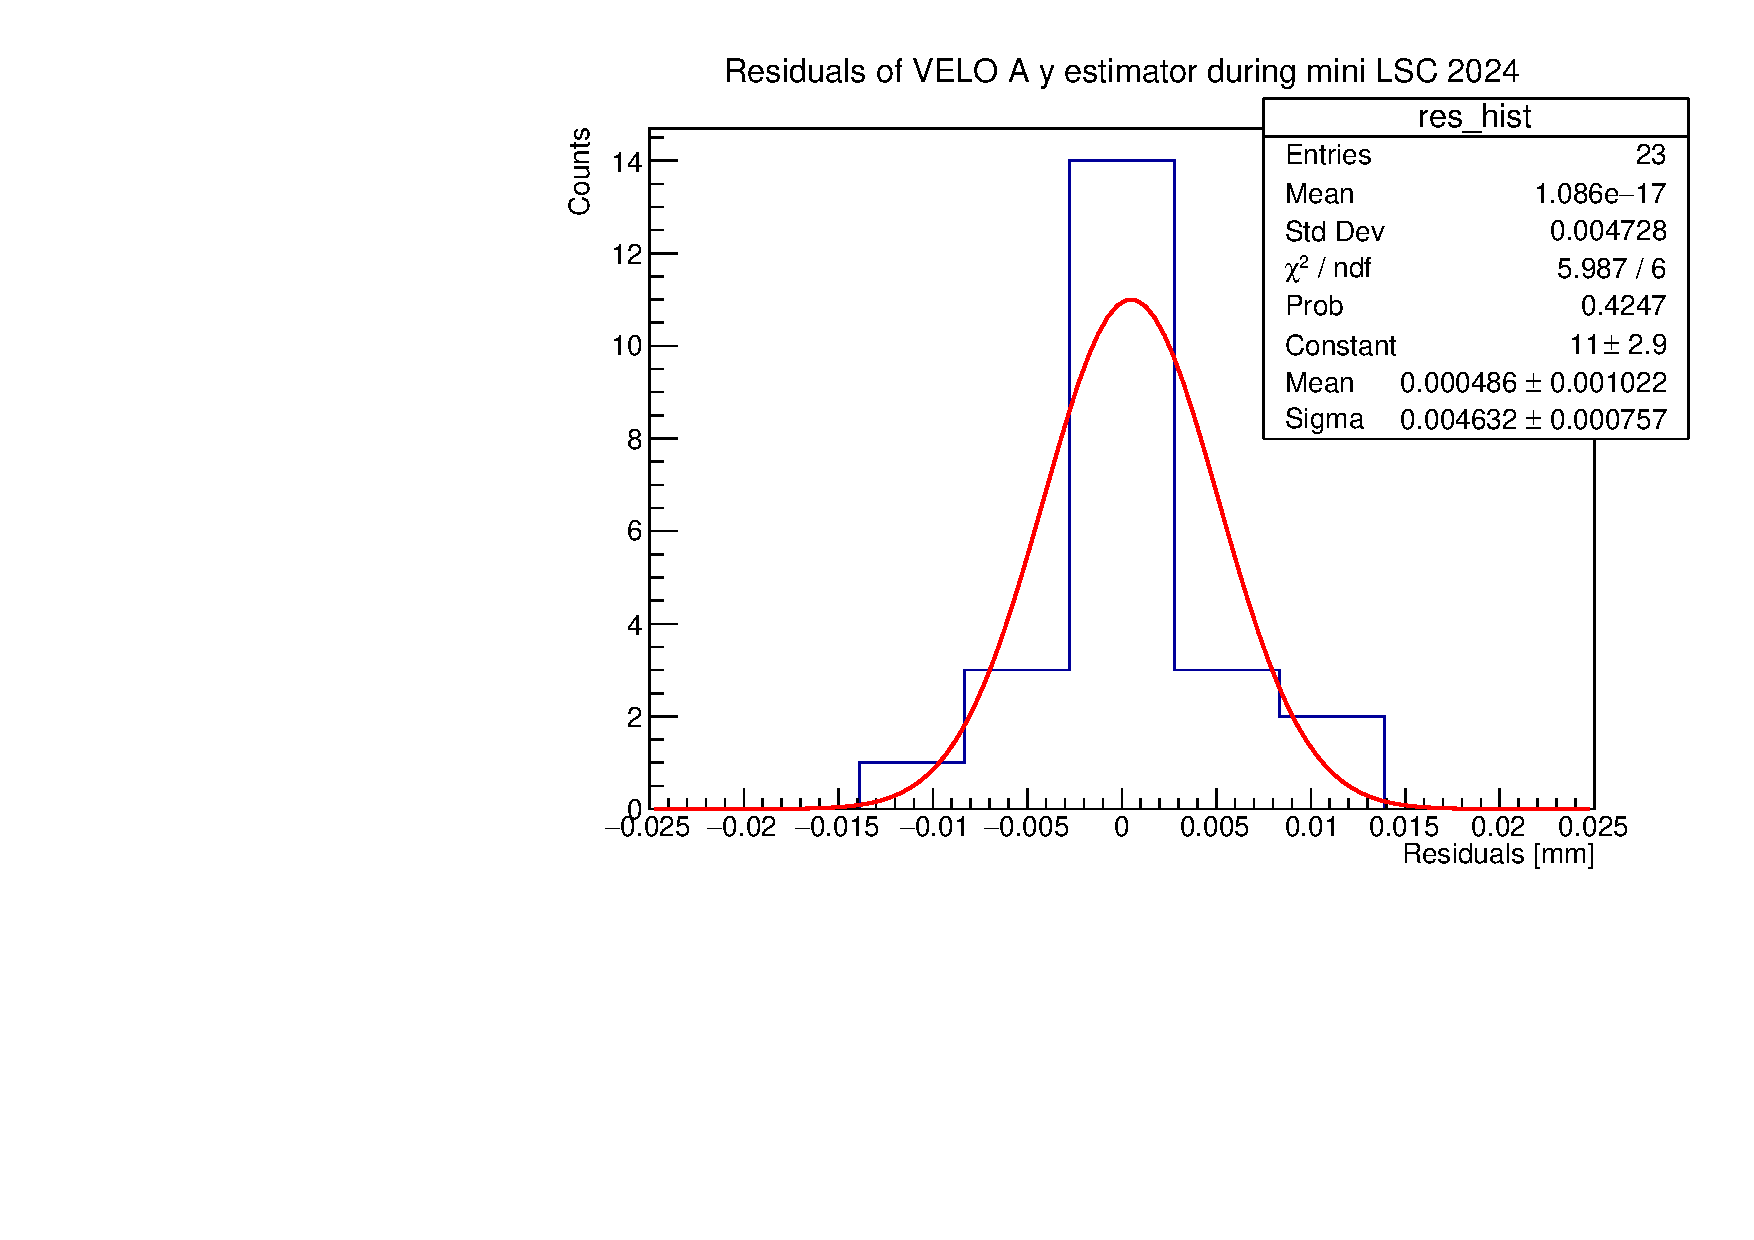
\includegraphics[width=\linewidth]{figures/y_res_VELO_A_data.pdf}
    \caption{Residuals from the fit of the graph on the left. }\label{fig:y_veloA_res_data}
    \end{subfigure}
    \caption{Linearity of the first component calculated with the PCA with respect to virtual VELO A position shifts in y component, alongside the residuals distribution fitted with a Gaussian distribution.}
    \label{fig:y_veloA_data}
\end{figure}



\begin{figure}
    \centering
    \begin{subfigure}{0.48\textwidth}
    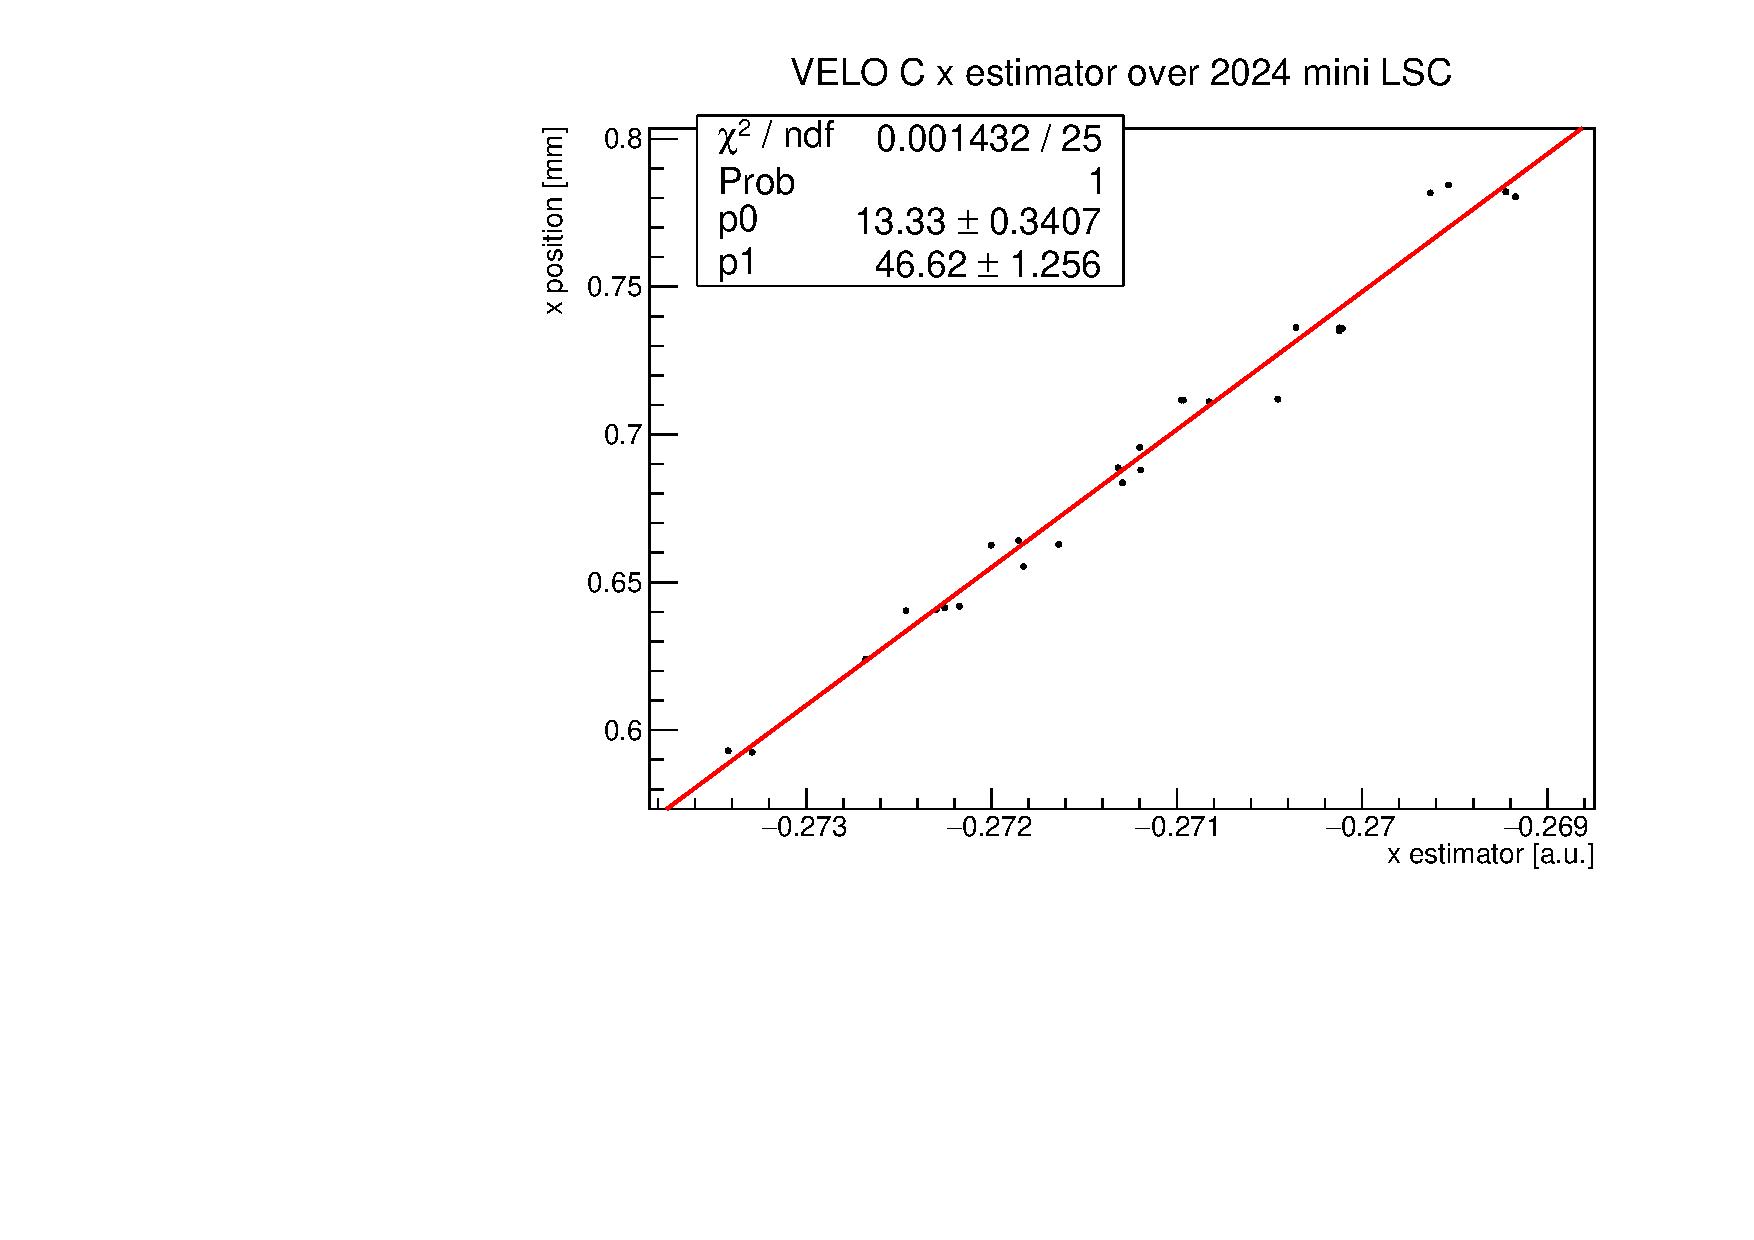
\includegraphics[width=\linewidth]{figures/x_fit_VELO_C_data.pdf}
    \caption{Linear Fit}\label{fig:x_veloC_fit_data}
    \end{subfigure}
    \begin{subfigure}{0.48\textwidth}
    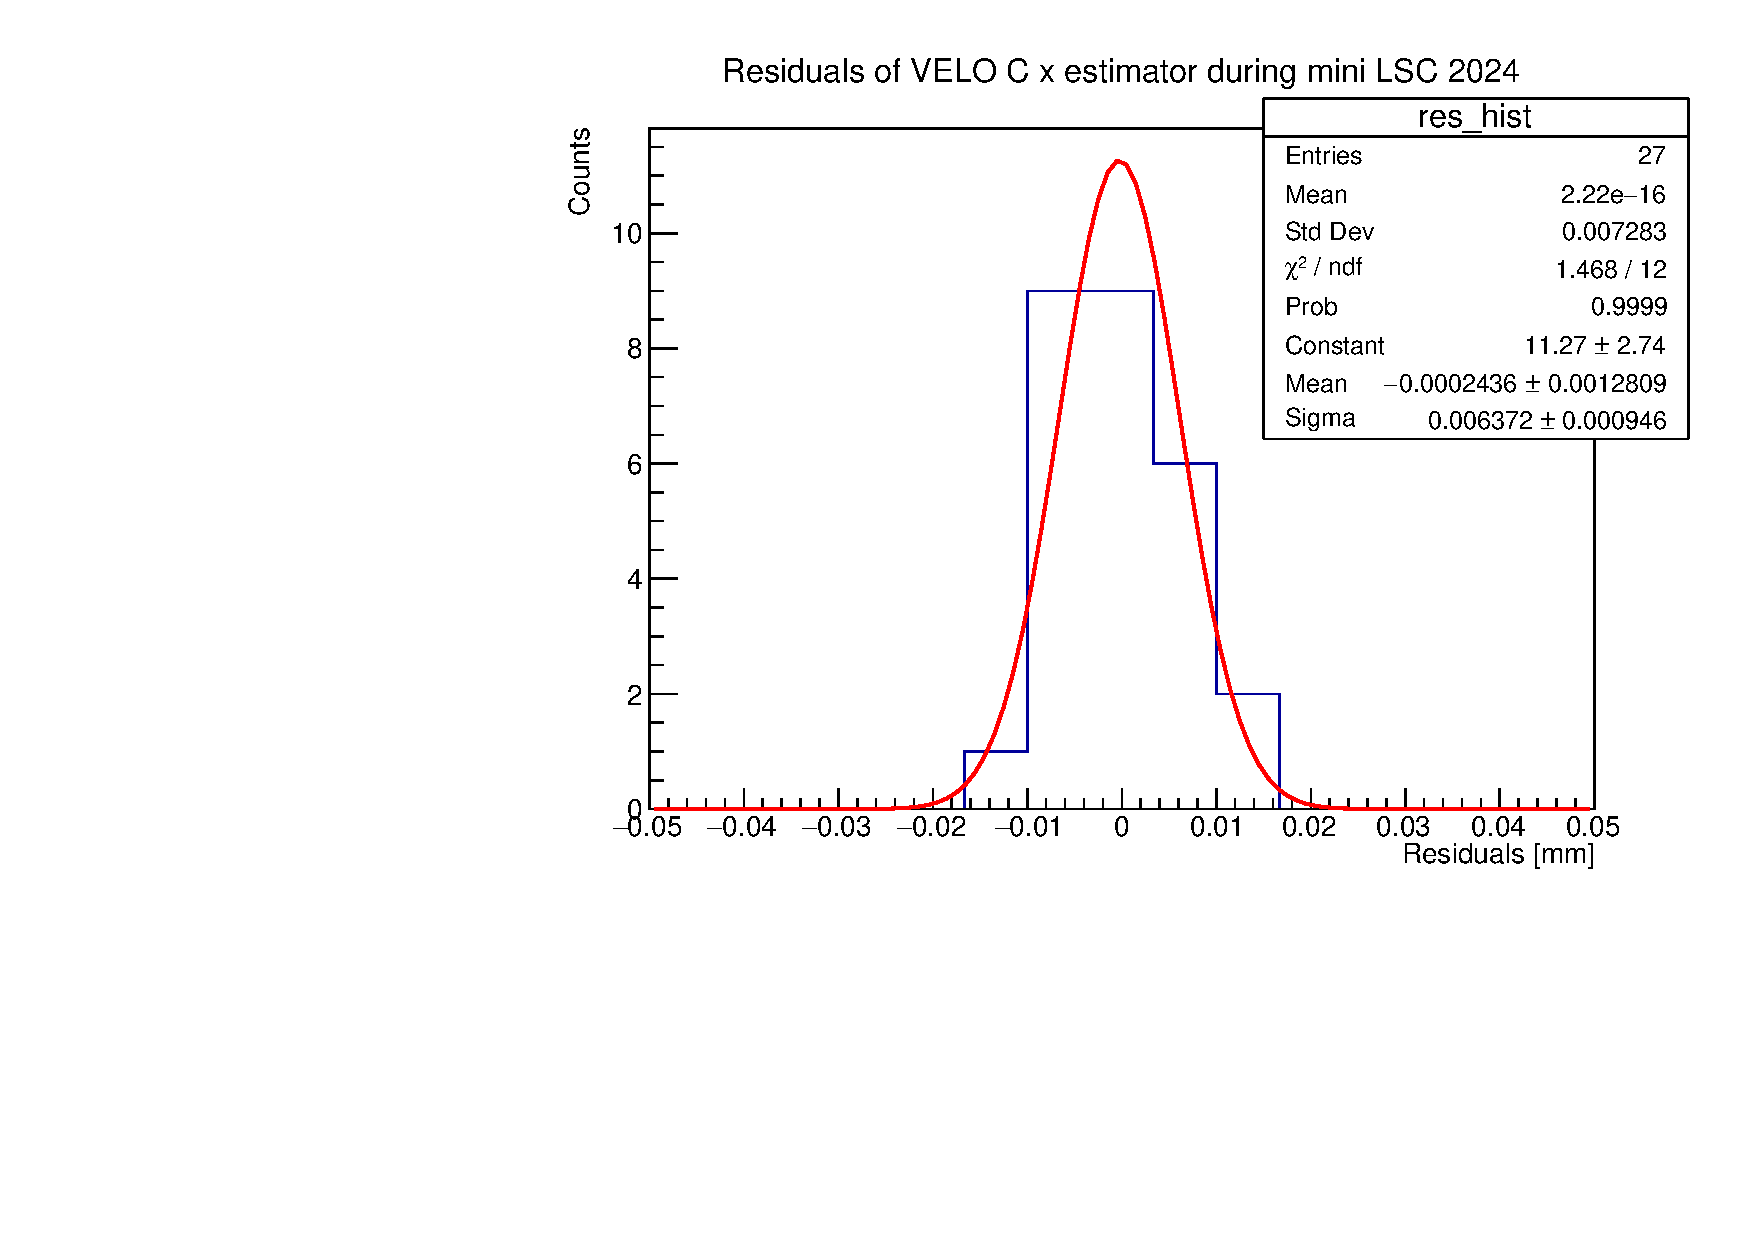
\includegraphics[width=\linewidth]{figures/x_res_VELO_C_data.pdf}
    \caption{Residuals from the fit of the graph on the left. }\label{fig:x_veloC_res_data}
    \end{subfigure}
    \caption{Linearity of the first component calculated with the PCA with respect to  virtual VELO C position shifts in x component, alongside the residuals distribution fitted with a Gaussian distribution.}
    \label{fig:x_veloC_data}
\end{figure}
\begin{figure}
    \centering
    \begin{subfigure}{0.48\textwidth}
    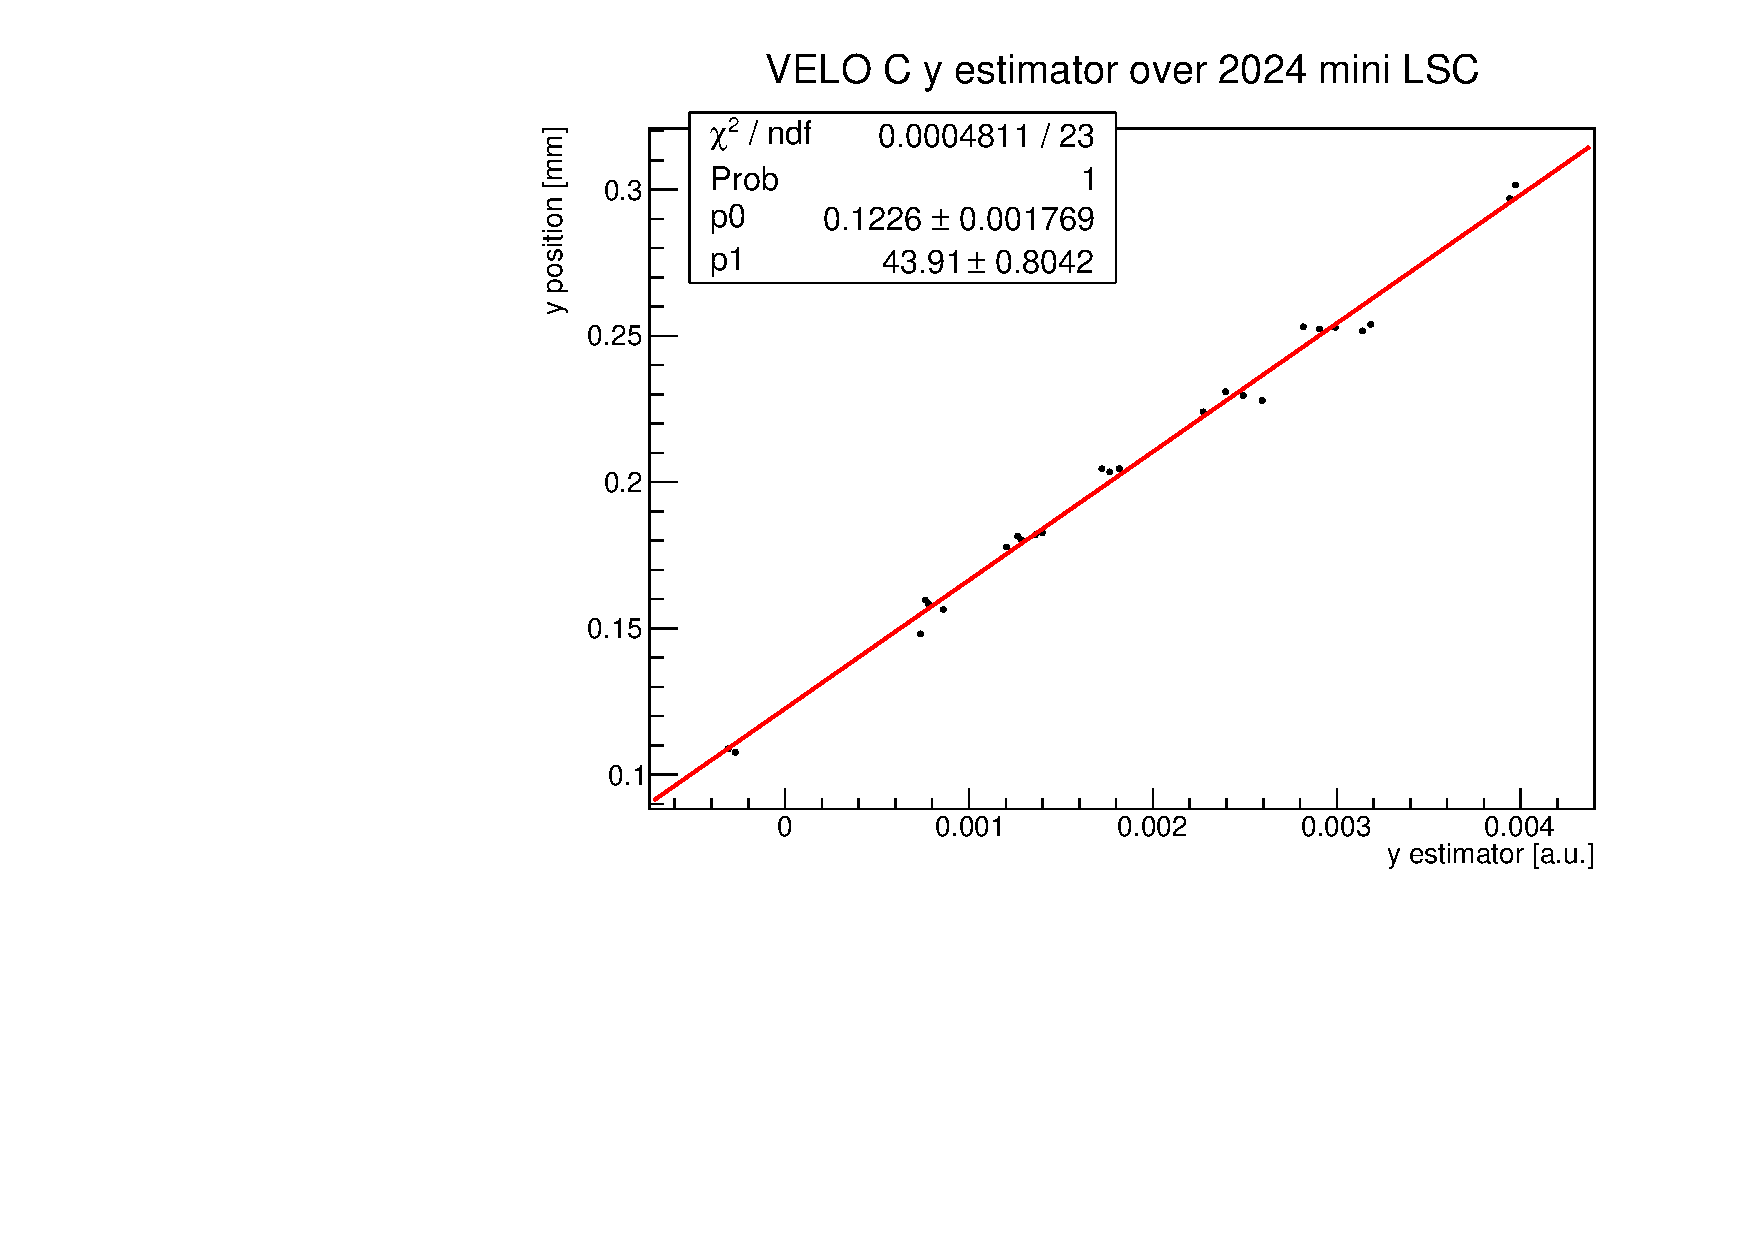
\includegraphics[width=\linewidth]{figures/y_fit_VELO_C_data.pdf}
    \caption{Linear Fit}\label{fig:y_veloC_fit_data}
    \end{subfigure}
    \begin{subfigure}{0.48\textwidth}
    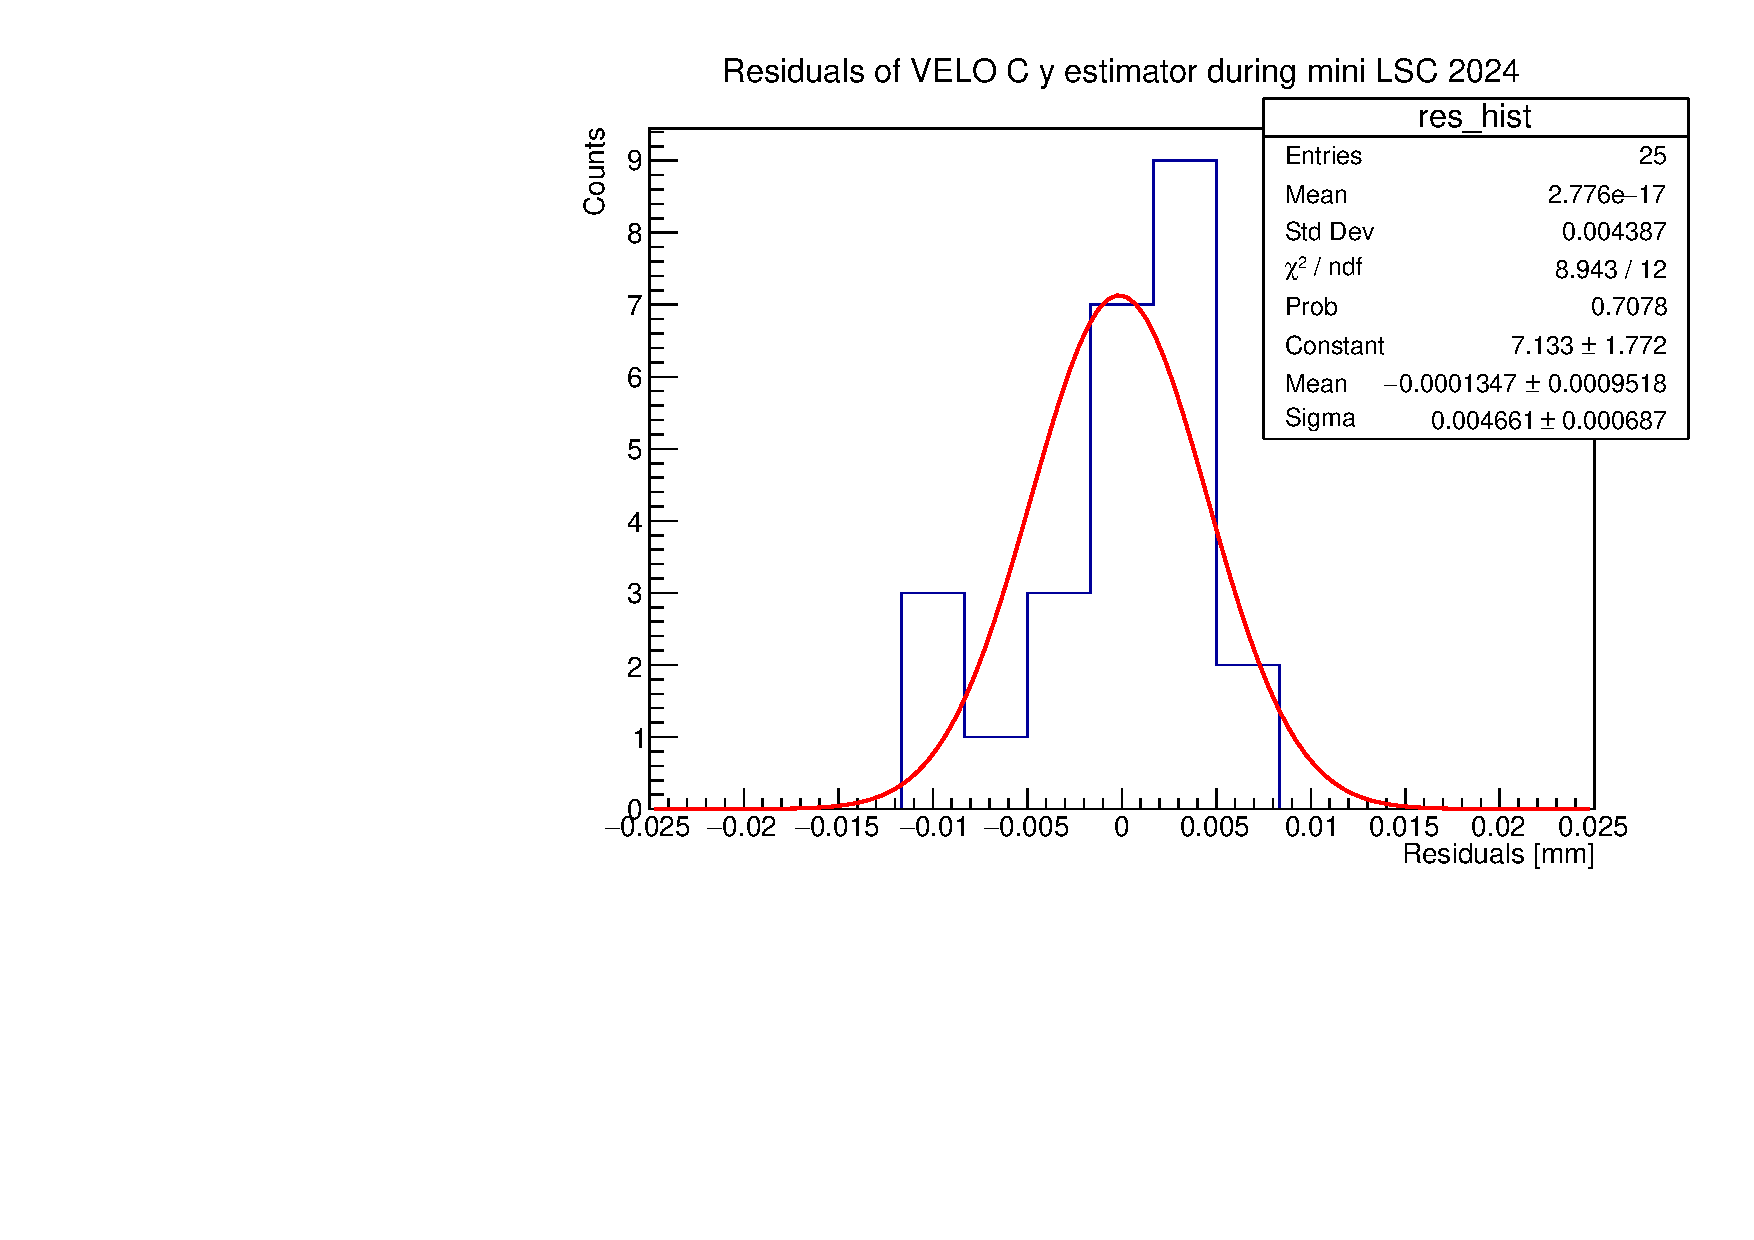
\includegraphics[width=\linewidth]{figures/y_res_VELO_C_data.pdf}
    \caption{Residuals from the fit of the graph on the left. }\label{fig:y_veloC_res_data}
    \end{subfigure}
    \caption{Linearity of the first component calculated with the PCA with respect to  virtual VELO C position shifts in y component, alongside the residuals distribution fitted with a Gaussian distribution.}
    \label{fig:y_veloC_data}
\end{figure}

The scatter plots alongare reported in the Figures \ref{fig:x_veloA_data}, \ref{fig:y_veloA_data}, \ref{fig:x_veloC_data}, \ref{fig:y_veloC_data}, respectively for $\hat{x}_A$, $\hat{y}_A$, $\hat{x}_C$, $\hat{y}_C$. As we can see from these scatter plot the relationship is linear, and from these fitted line we can infer the parameters that allows to calculate the estimators $\hat{x}_A$, $\hat{y}_A$, $\hat{x}_C$, $\hat{y}_C$.

In Figure \ref{fig:traceplot_xy}, we report the traceplot of the estimators during a the two LSC. The relationship is 

\begin{figure}
    \centering
    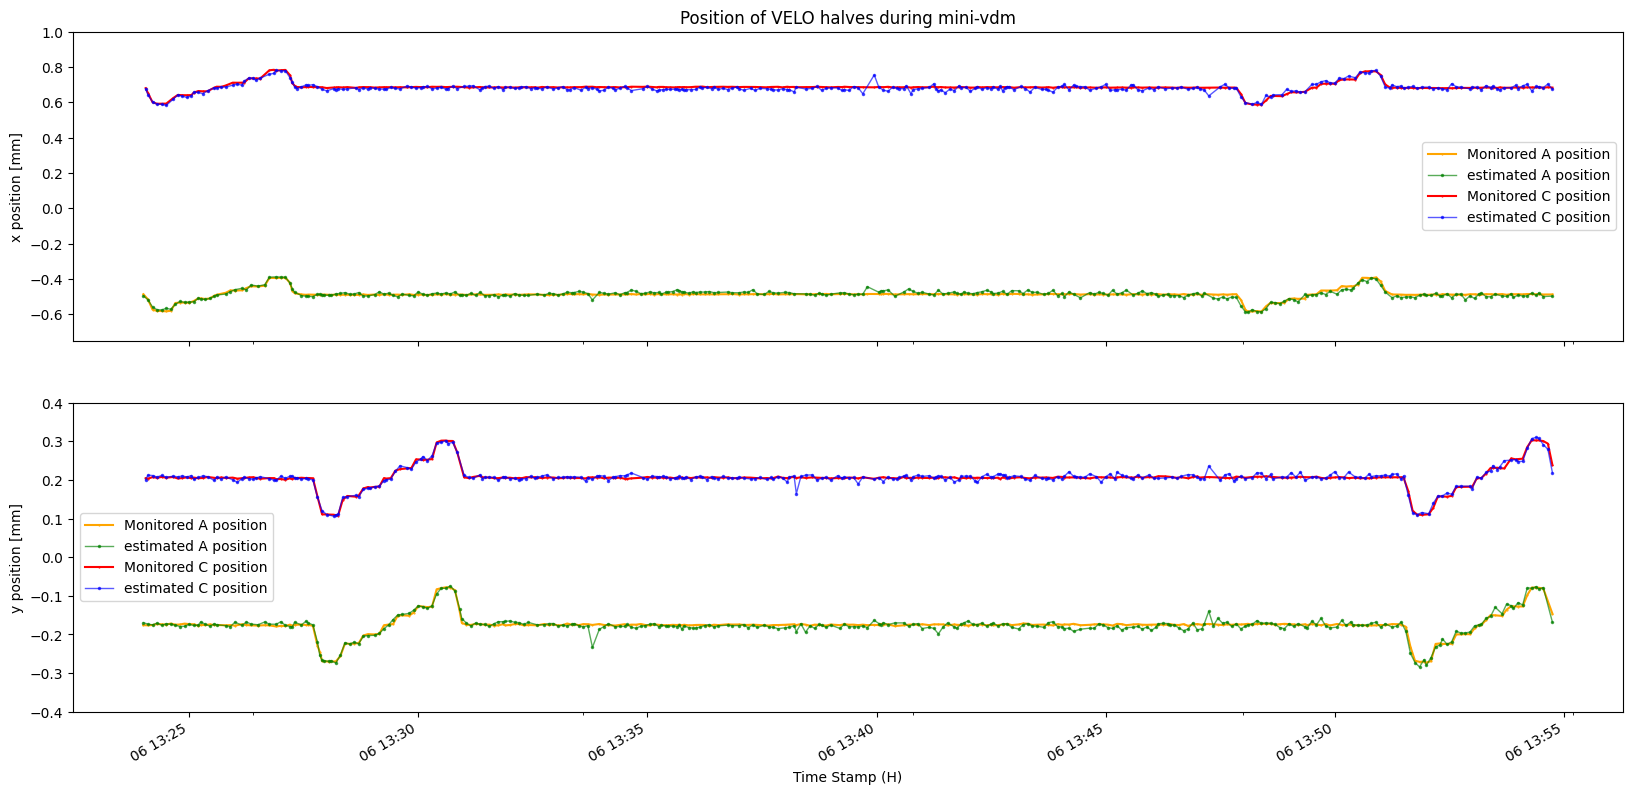
\includegraphics[width=\textwidth]{figures/traceplot_xy.png}
    \caption{Caption}
    \label{fig:traceplot_xy}
\end{figure}

\section{A testing scenario: monitoring the VELO drift}
